\section{Kernel Troubles}
During the analysis it became clear, that the data model obtained through the debug symbols is far from perfect.
This is due to C language issues and the tendency of developers to use type-casting macros, which override the data model obtained through the debug images.
This section is going to discuss several problem areas we came across and shows ideas on how to work around them.

\subsection{Kernel Symbols}
Kernel symbols associate a memory address with a \texttt{Variable} instance (and thus a name) which is known through the \texttt{objdump} output.
However, not all kernel symbols are contained in the kernel image itself.
This is partly due to the fact, that several symbols are not available at the time the kernel is built, but are hacked into the kernel after the main build process.

The kernel itself contains a complete symbol table which is used, for example, for loadable modules.
Unfortunately this table is stored compressed in memory and its address is also not yet known at build-time.
While it would seem reasonable to use heuristics to find this symbol table and implement the algorithm to decompress it, the easiest approach is to just read all those symbols from either the proc-filesystem or the \texttt{System.map} which should be available in most scenarios.

\subsection{Linked Lists}
\label{sec:linkedlists}
Linked lists are a central data structure used in many places throughout the kernel and there is a standard implementation of preprocessor macros facilitating the use of linked lists in kernel code.
These lists are actually very basic and only become powerful when instrumented by those macros.
Listing \ref{lst:linkedlists} illustrates the common usage, where the generic \texttt{list\_head} is embedded into another data-structure.
\begin{lstlisting}[frame=single,caption=Linked lists as used in the linux kernel,label=lst:linkedlists]
//  | next | -->  | next | -->  | first | 
//  | last |  <-- | prev |  <-- | prev  |
struct list_head {
        struct list_head *next, *prev;
};
struct data {
        int attribute;
        struct list_head list;
};
struct data * some_data;
struct data * sample = list_entry(some_data->list.next, struct data, list);
\end{lstlisting}
The problem arises when list-members are accessed: \texttt{some\_data->list.next} points to the \texttt{list} attribute in another instance of \texttt{struct data}.
As such our tool will be able to follow the linked list itself, but is not able to determine, that the entries actually belong to \texttt{struct data} instances.
Thus without further work, the tool would miss data. This cannot be afforded with data structures so frequently used as linked lists.
In order to be able to follow the reference to the parent, it would be required to know the parent structure and its \texttt{struct list\_head} member for the very memory location that \texttt{list.next} points to.
Unfortunately this information is not available.

A successful heuristic for some of these cases is, that \texttt{list.next} always points to a \texttt{list\_head}-instance embedded in another instance of the same type
(i.e.~\texttt{data.list.next} always points to a \texttt{struct list\_head list} member in \texttt{struct data} in the example).
This allows us to implement a meta-type for \texttt{list\_head}-members in structures and handle those in such a way that they will recalculate the position when following a next or prev pointer,
which is also what the macros do (i.e.~\texttt{list\_entry(pointer, structure, attribute)} in listing \ref{lst:linkedlists}).
However, these macros are given explicit advice on what attribute in which data structure is referenced by the pointer.
With the meta-type modification in place, the data model will no longer show \texttt{data.list.next} pointing to an instance of \texttt{struct list\_head}, but will show it pointing directly to the next \texttt{struct data} instance.

While this covers some amount of the actual uses of linked lists in the kernel, there are a lot of notable exceptions in which the heuristic is not applicable.
Often entry points to linked lists are stored in global variables or structures having nothing to do with the linked list at all.
Another example of unconventional use of linked lists are structures with multiple lists such as \texttt{struct task\_struct}
whose \texttt{children} attribute is actually a linked-list pointing to the \texttt{sibling} attribute in another \texttt{task\_struct}.
Since the manual tracking of such exceptions is time-consuming, we rather tried to automate this task.

\paragraph{Automated source-code based information acquirement}
We implemented the non-manual approach that we already had in mind earlier but originally assumed the hurdles for an actual implementation to be to hard to overcome.
The approach looks for usages of linked-list related macros on a source-code level and can then establish relationships between members and referenced data structures.
The scanning of the source-code is based on regular expressions and relies largely on the rather clean coding style used by the kernel programmers.
The biggest trouble is then to discover the types of the involved variables.
However, with the library for accessing debuging symbols already at hand, this becomes feasible.
The remaining task is to reconstruct the data model according to the references established through the analysis.
\begin{lstlisting}[frame=single,caption=Linked lists referencing other types (excerpt from kernel/exit.c),label=lst:linkedliststypes]
void mm_update_next_owner(struct mm_struct *mm)
{
    struct task_struct *c, *p = current;

    list_for_each_entry(c, &p->children, sibling) {
        ...
    }
    ...
}
\end{lstlisting}
\begin{figure}[htb]
    \begin{center}
    %dia export to pango-eps, then
    % ps2pdf task_struct_illustration.eps
    % pdfcrop task_struct_illustration.pdf
	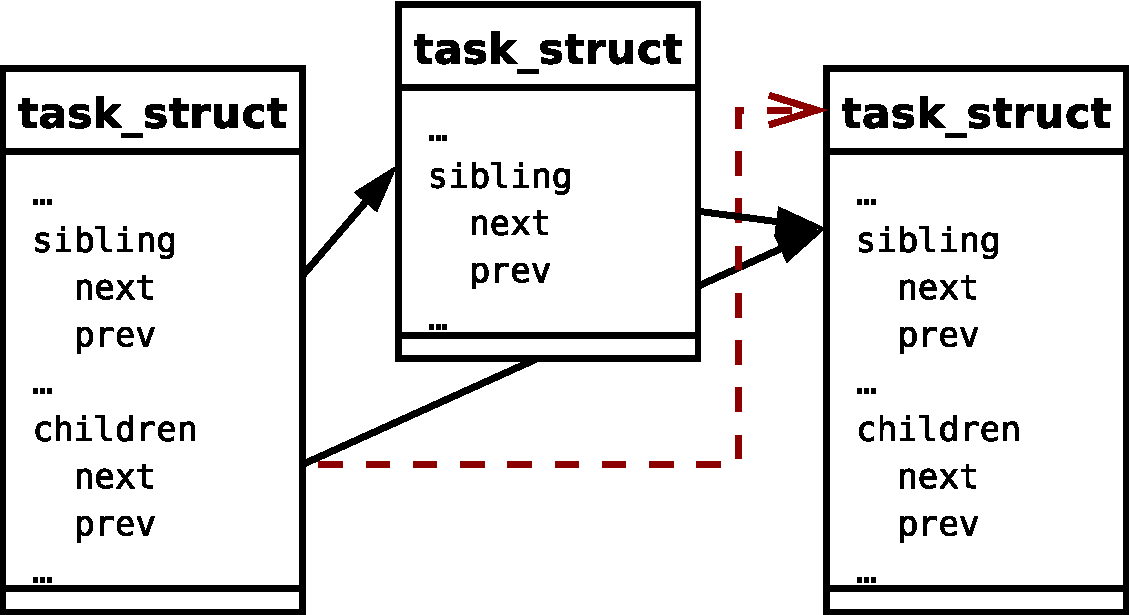
\includegraphics[width=8cm]{imgs/task_struct_illustration-crop.pdf}
    \end{center}
	
	\caption{Illustration of references used by linked lists in a \texttt{task\_struct}}
	\label{fig:task-struct-image}
\end{figure}
The example in listing \ref{lst:linkedliststypes} and figure \ref{fig:task-struct-image} can be used to illustrate the procedure:
A loop over all elements in a list is a frequent task.
\texttt{c} is the current element and its type \texttt{struct task\_struct} is the target object, i.e.~after the process, the tool should be able to do pointer magic such that \texttt{children.next} points to a \texttt{struct task\_struct}.
For now we do not know that \texttt{children.next} points to the \texttt{sibling} attribute of a \texttt{struct task\_struct}.
The usage of the macro however gives us the information: the last parameter is the name of the attribute inside the destination type.
The second attribute \texttt{\&p->children} gives us information for which member this association will be valid.
Again we use the debug symbols to find out that \texttt{p} is a \texttt{struct task\_struct} whose \texttt{children}’s attribute is then accessed.
\newline
Using this procedure, the mapping from \texttt{task\_struct.children} to \texttt{task\_struct.sibling} is established.
When accessing \texttt{children.next} we then know, that the pointer needs to be modified to subtract the offset of \texttt{sibling} within \texttt{task\_struct} to get a pointer to an actual \texttt{task\_struct}.

This approach yields considerable results: out of roughly 700 linked-lists 300 are auto-associated and the 
regular-expression based source-lookup tool could still be improved a lot to increase coverage. Nevertheless, 
there are a number of remaining structures for which the self-referencing heuristic mentioned earlier might 
not be valid and to which we do not gain access.

\subsection{Hashtables}
Even more troublesome than linked lists are hashtables, because the simple heuristics that have been helpful for linked-lists cannot be applied.
A hashtable is usually an array of \texttt{struct hlist\_head} elements which are entry elements (pointers) to a linked list of items in this bucket of the hashtable.
Each such item is represented by a \texttt{hlist\_node} structure which is a linked list similar to the \texttt{list\_head} structure. These nodes are also embedded into other data structures.
\begin{lstlisting}[frame=single,caption=Headed linked lists as used in the linux kernel,label=lst:hlists]
// first --> | next | -->  | next | -->  | next | 
//           | prev |  <-- | prev |  <-- | prev |
\end{lstlisting}
However there is no reference which structures belong to the \texttt{hlist\_node}s of a given hashtable array.
As it turns out though, the usage of the macro \texttt{void hlist\_add\_head(struct hlist\_node *n, struct hlist\_head *h)} establishes a connection between a \texttt{hlist\_head} instance and the corresponding \texttt{hlist\_node} structure.
While this macro and its use is not accessible from the debug symbols, it is quite grepable from the source.
We did not yet implement an automated approach, but feel confident that the same techniques we used to auto-associate linked lists can be used here to auto-associate the corresponding parent structures
(those that include \texttt{hlist\_head}, \texttt{hlist\_node}).
We can then use the generated mapping to implement an abstract Hashtable data type that takes these specialities into account.
Also a manual approach might succeed, as it seems there are less than 50 different hashtables in the kernel.

As long as the hashtable-handling has not been implemented, heuristic workarounds may be used, % in the meantime,
although these dirty approaches have significant drawbacks and should only be used to overcome the time until the hashtable-mappings are present.
There is an upper bound for structures including those hashtable nodes, which never exceed 2048 bytes.
Thus while the specific semantics of a memory region belonging to a \texttt{struct hlist\_node} are unknown,
it is known that up to 2048 bytes are being used to store information. As such, comparing memory can go ahead and compare the raw bytes,
trying to find out what changed.
Unfortunately all hashtable nodes also contain pointers, indicating that there is more information belonging to a node and that this information is not stored within the node itself.
Since the semantics of the memory region are unknown, we are likely to miss entry points to other memory structures when restricting hashtable node comparison to the very local memory only.

Hashtables in the kernel are usually used to store data, but most likely do not store very sensitive data or provide entry points to huge memory regions which would be missed if the references from the hashtable would not be followed.
As such it seems reasonable to skip hashtable handling in a first approach completely.

\subsection{Arrays and Pointers}
It is common convention to declare Strings as \texttt{char}-pointers (\texttt{char *}), however in the data model, a \texttt{char *} is a pointer to a \texttt{BasicType} instance \texttt{char} which is exactly one byte long.
While this knowledge is used to convert all \texttt{char}-pointers to a String meta-type, it is not clear what should be the behaviour for other types, as \texttt{int *} might also reference an integer field.
However, even if the integer field is correctly declare as \texttt{int field[]}, the length is still unknown,
leaving it for the program to guess or \emph{know}.
There seems no easy way to overcomes this problem, but to ignore all the data in the field unless one uses manual approaches:
Usually the array’s length is indirectly known: be it a static configuration or another member of a \texttt{struct}.
It is then no problem to override the array’s length by type-casting to an \texttt{Array} of a specified length.
There is also a \texttt{NullTerminatedArray} class which assumes a \texttt{NULL} entry to be the end delimiter,
which might be the case for many of those arrays with unknown length information.
